\newpage
\chapter{Mission}
The purpose of these functions is to simulate a mission with certain accuracy and to configure an engine based on the required mission.
\section{Update chamber functions}
The following functions were built to have an easy call in the main mission function to update pressure and thermodynamic properties at every step. Available in \textit{Mission//chamber\_update.py}.

\begin{verbatim}
find_dt(Tc, MW, gamma, Tc_CEA, MW_CEA, gamma_CEA, 
m_c_i, Dmdot_in, Dmdot_out, tol=1e-3)
-> return dt
\end{verbatim}
\hspace*{2em} Called inside the next function, returns the needed time step to have a variation in the thermodynamic properties under the required tolerance. It is calculated using the mixture of gases formulas:
\begin{gather}
    \begin{matrix}
        m_{i+1}=m_i-\dot{m}_{out}dt+\dot{m}_{in}dt\\
        c_{p,i+1}=\frac{(m_i-\dot{m}_{out}dt)c_{p,i}+\dot{m}_{in}dtc_{p,CEA}}{m_{i+1}}\\
        T_{c,i+1}=\frac{(m_i-\dot{m}_{out}dt)T_{c,i}c_{p,i}+\dot{m}_{in}dtT_{c,CEA}c_{p,CEA}}{m_{i+1}}\\
        MW_{i+1}=\frac{m_{c,i+1}}{\frac{m_i-\dot{m}_{out}dt}{MW_i}+\frac{\dot{m}_{in}dt}{MW_{CEA}}}
    \end{matrix}
    \label{Eq: MixGas}
\end{gather}
Setting a relative tolerance for the generic value
\begin{equation}
    |\frac{X_i+1}{X_i}-1|=tol
\end{equation}
we can finally find four different time-steps, leading us to the decision of taking the minimum one.

\begin{verbatim}
update_Temperature_and_gasproperties(pc, Tc, MW, gamma, Tc_CEA, MW_CEA, 
gamma_CEA, mdot_ox, mdot_fuel, mdot_throat, Vol_chamber, tol=1e-3)
-> return Tc_actual, MW_actual, gamma_actual, m_c, dt
\end{verbatim}
\hspace*{2em} Calculates new gas properties using ideal gas state equation and mixture of gases relations in \ref{Eq: MixGas}. The first step is to calculate the mass of fluid inside the chamber
\begin{equation}
    m_i=\frac{p_{c,i}V_i}{R_iT_{c,i}}
\end{equation}
we get the time-step with \verb|find_dt(...)| and then apply the \ref{Eq: MixGas}.\\
What should be considered while reading the results is that while the ideal gas assumption could be acceptable, the results to update the values are taken from NASA CEA \cite{NASACEA}, which considers the reaction in chemical equilibrium with infinite residence time and does not consider transitory effects due to finite distances and times. This makes this model less-accurate than a proper CFD with reactive species but allows to use a vast database of possible reactants. The main solution is to validate the output through static-fires, determining performances' efficiencies and using them for better prediction.

\begin{verbatim}
update_chamberpressure(m_c, Tc, MW, Vol_chamber)
-> return pc
\end{verbatim}
\hspace*{2em} Calculates the new chamber pressure using ideal gas state equation with updated values.

\section{Simulation functions}
The following functions are intended to fully simulate a mission using required times and injection or burning conditions. Available in \textit{Mission//mission\_simulation.py}.

\begin{verbatim}
find_nozzle_output(gamma, MW, Tc, pc, mdot_throat, pamb, At, eps)
return Me, Te, pe, Ve
\end{verbatim}
\hspace*{2em} calculates the properties at the exit section of the nozzle, needed to calculate the thrust.\\
We determine if the nozzle is chocked when
\begin{equation}
    \frac{p_{amb}}{p_c}<(\frac{p_e}{p_c})_{crit}=(\frac{2}{\gamma+1})^{\frac{\gamma}{\gamma-1}}
\end{equation}
but actually this relation is valid if we look for a chocked exit section. The real condition is a critical throat section, from mass conservation we get
\begin{equation}
    f(\frac{p_{amb}}{p_c})\geq \frac{f(M=1)}{\varepsilon}
\end{equation}
If one of the two conditions is satisfied, we iteratively find exit section Mach number using mass flow conservation and mach function equation to create the target function
\begin{equation}
    F(M_e)= f(M_e) - \dot{m}_{t} \frac{\sqrt{RT_c}}{p_cA_t\varepsilon}=0
\end{equation}
with
\begin{equation*}
    f(M)= \frac{\sqrt{\gamma}M}{\sqrt{(1+\frac{\gamma-1}{2}M^2)^{\frac{\gamma+1}{\gamma-1}}}}
\end{equation*}
We use Newton's method, calculating the derivative of Mach function
\begin{equation}
    \frac{df}{dM}=\sqrt{\gamma}(\frac{1}{\sqrt{(1+\frac{\gamma-1}{2}M^2)^{\frac{\gamma+1}{\gamma-1}}}} -\frac{\gamma+1}{2}M^2 \frac{(1+\frac{\gamma-1}{2}M^2)^{\frac{2}{\gamma-1}}}{\sqrt{(1+\frac{\gamma-1}{2}M^2)^{3\frac{\gamma+1}{\gamma-1}}}})
\end{equation}
After finding the exit Mach number we calculate the needed values using the adiabatic flow equations
\begin{gather}
    \begin{matrix}
        \frac{T_c}{T_e}=1+\frac{\gamma-1}{2}M^2\\
        \frac{p_c}{p_e}=(1+\frac{\gamma-1}{2}M^2)^{\frac{\gamma}{\gamma-1}}\\
        v=M\sqrt{\gamma RT_c}
    \end{matrix}
    \label{Eq: Adiab}
\end{gather}
If the nozzle is not chocked we assume
\begin{equation}
    p_e=p_{amb}
\end{equation}
and use the \ref{Eq: Adiab}.

\begin{verbatim}
get_starting_conditions(pamb, Tamb, rho_fuel, x, y, Lc, D_chamber, 
Vol_prechamber, Vol_postchamber, masses, volumes, pressures, temperatures, 
oxidizer, pressurant=None, pitch=0.0, circular=False, 
npointsperside=50, constant_pressure_tank=False)
-> return (pc, mdot_throat, Tc, MW, gamma,
            ptank, Ttank, mL, m_fuel,
            entropies, masses, pressures, temperatures,
            Ap, Ab, Vol_chamber)
\end{verbatim}
\hspace{2em} Sets starting pressure, temperature and properties equal to ambient's (CoolProp's Air), gets tank starting conditions with \verb|start_conditions(...)|, calculates port area, burning area and chamber volume with \verb|fill_and_calculate_surfaces_and_volume(...)| and the fuel mass with \verb|calculate_fuel_mass(...)|.

\begin{verbatim}
run_one_step_no_burn(pc, mdot_throat, Tc, MW, gamma, rho_fuel, pamb, ptank, 
Ttank, eps, Ainj, At, Ap, Ab, Lc, Vol_chamber, D_chamber, x, y, 
entropies, masses, volumes, pressures, temperatures, utilities, CD, oxidizer,
pressurant=None, rend_CF = 1.0, constant_pressure_tank=False, tol=1e-3)
-> return (pc, mdot_throat, Thrust, dt,
            Tc, MW, gamma, ptank, Ttank, eps,
            mL, m_fuel,
            Ap, Ab, Vol_chamber,
            x, y,
            entropies, masses, pressures, temperatures,
            performances)
\end{verbatim}

\begin{verbatim}
run_one_step(pc, mdot_throat, Tc, MW, gamma, a, n, rho_fuel, pamb, ptank, 
Ttank, eps, Ainj, At, Ap, Ab, Lc, Vol_chamber, Vol_prechamber, Vol_postchamber, 
D_chamber, x, y, z, entropies, masses, volumes, pressures, temperatures, utilities,
CD, oxidizer, fuel, pressurant=None, rend_cstar = 1.0, rend_CF = 1.0, pitch=0.0,
circular=False, npointsperside=50, constant_pressure_tank=False, tol=1e-3)
-> return (pc, mdot_throat, Thrust, dt,
            Tc, MW, gamma, ptank, Ttank, eps,
            mL, m_fuel,
            Ap, Ab, Vol_chamber,
            x, y,
            entropies, masses, pressures, temperatures,
            performances, flag)
\end{verbatim}

\hspace{2em} These two functions have the same output and are meant to be used inside an iteration (to have an easy call) and manage all the operations to update the values after one time-step. The explicit outputs are used directly in the next iteration or to control the termination, the implicit one \verb|performances| represents a dictionary with a series of important values to be given as an output. It's structure will be later discussed.
The workflow for the mission simulation is the one presented in Figure \ref{fig:flowchartstep}. The main difference between the burn and no-burn function are in point \textit{2)}, where only \verb|linelosses(...)| and \verb|massflow(...)| functions are used and the fluid properties are the oxidizer ones, and point \textit{4)}, that is skipped.
\begin{figure}
    \centering
    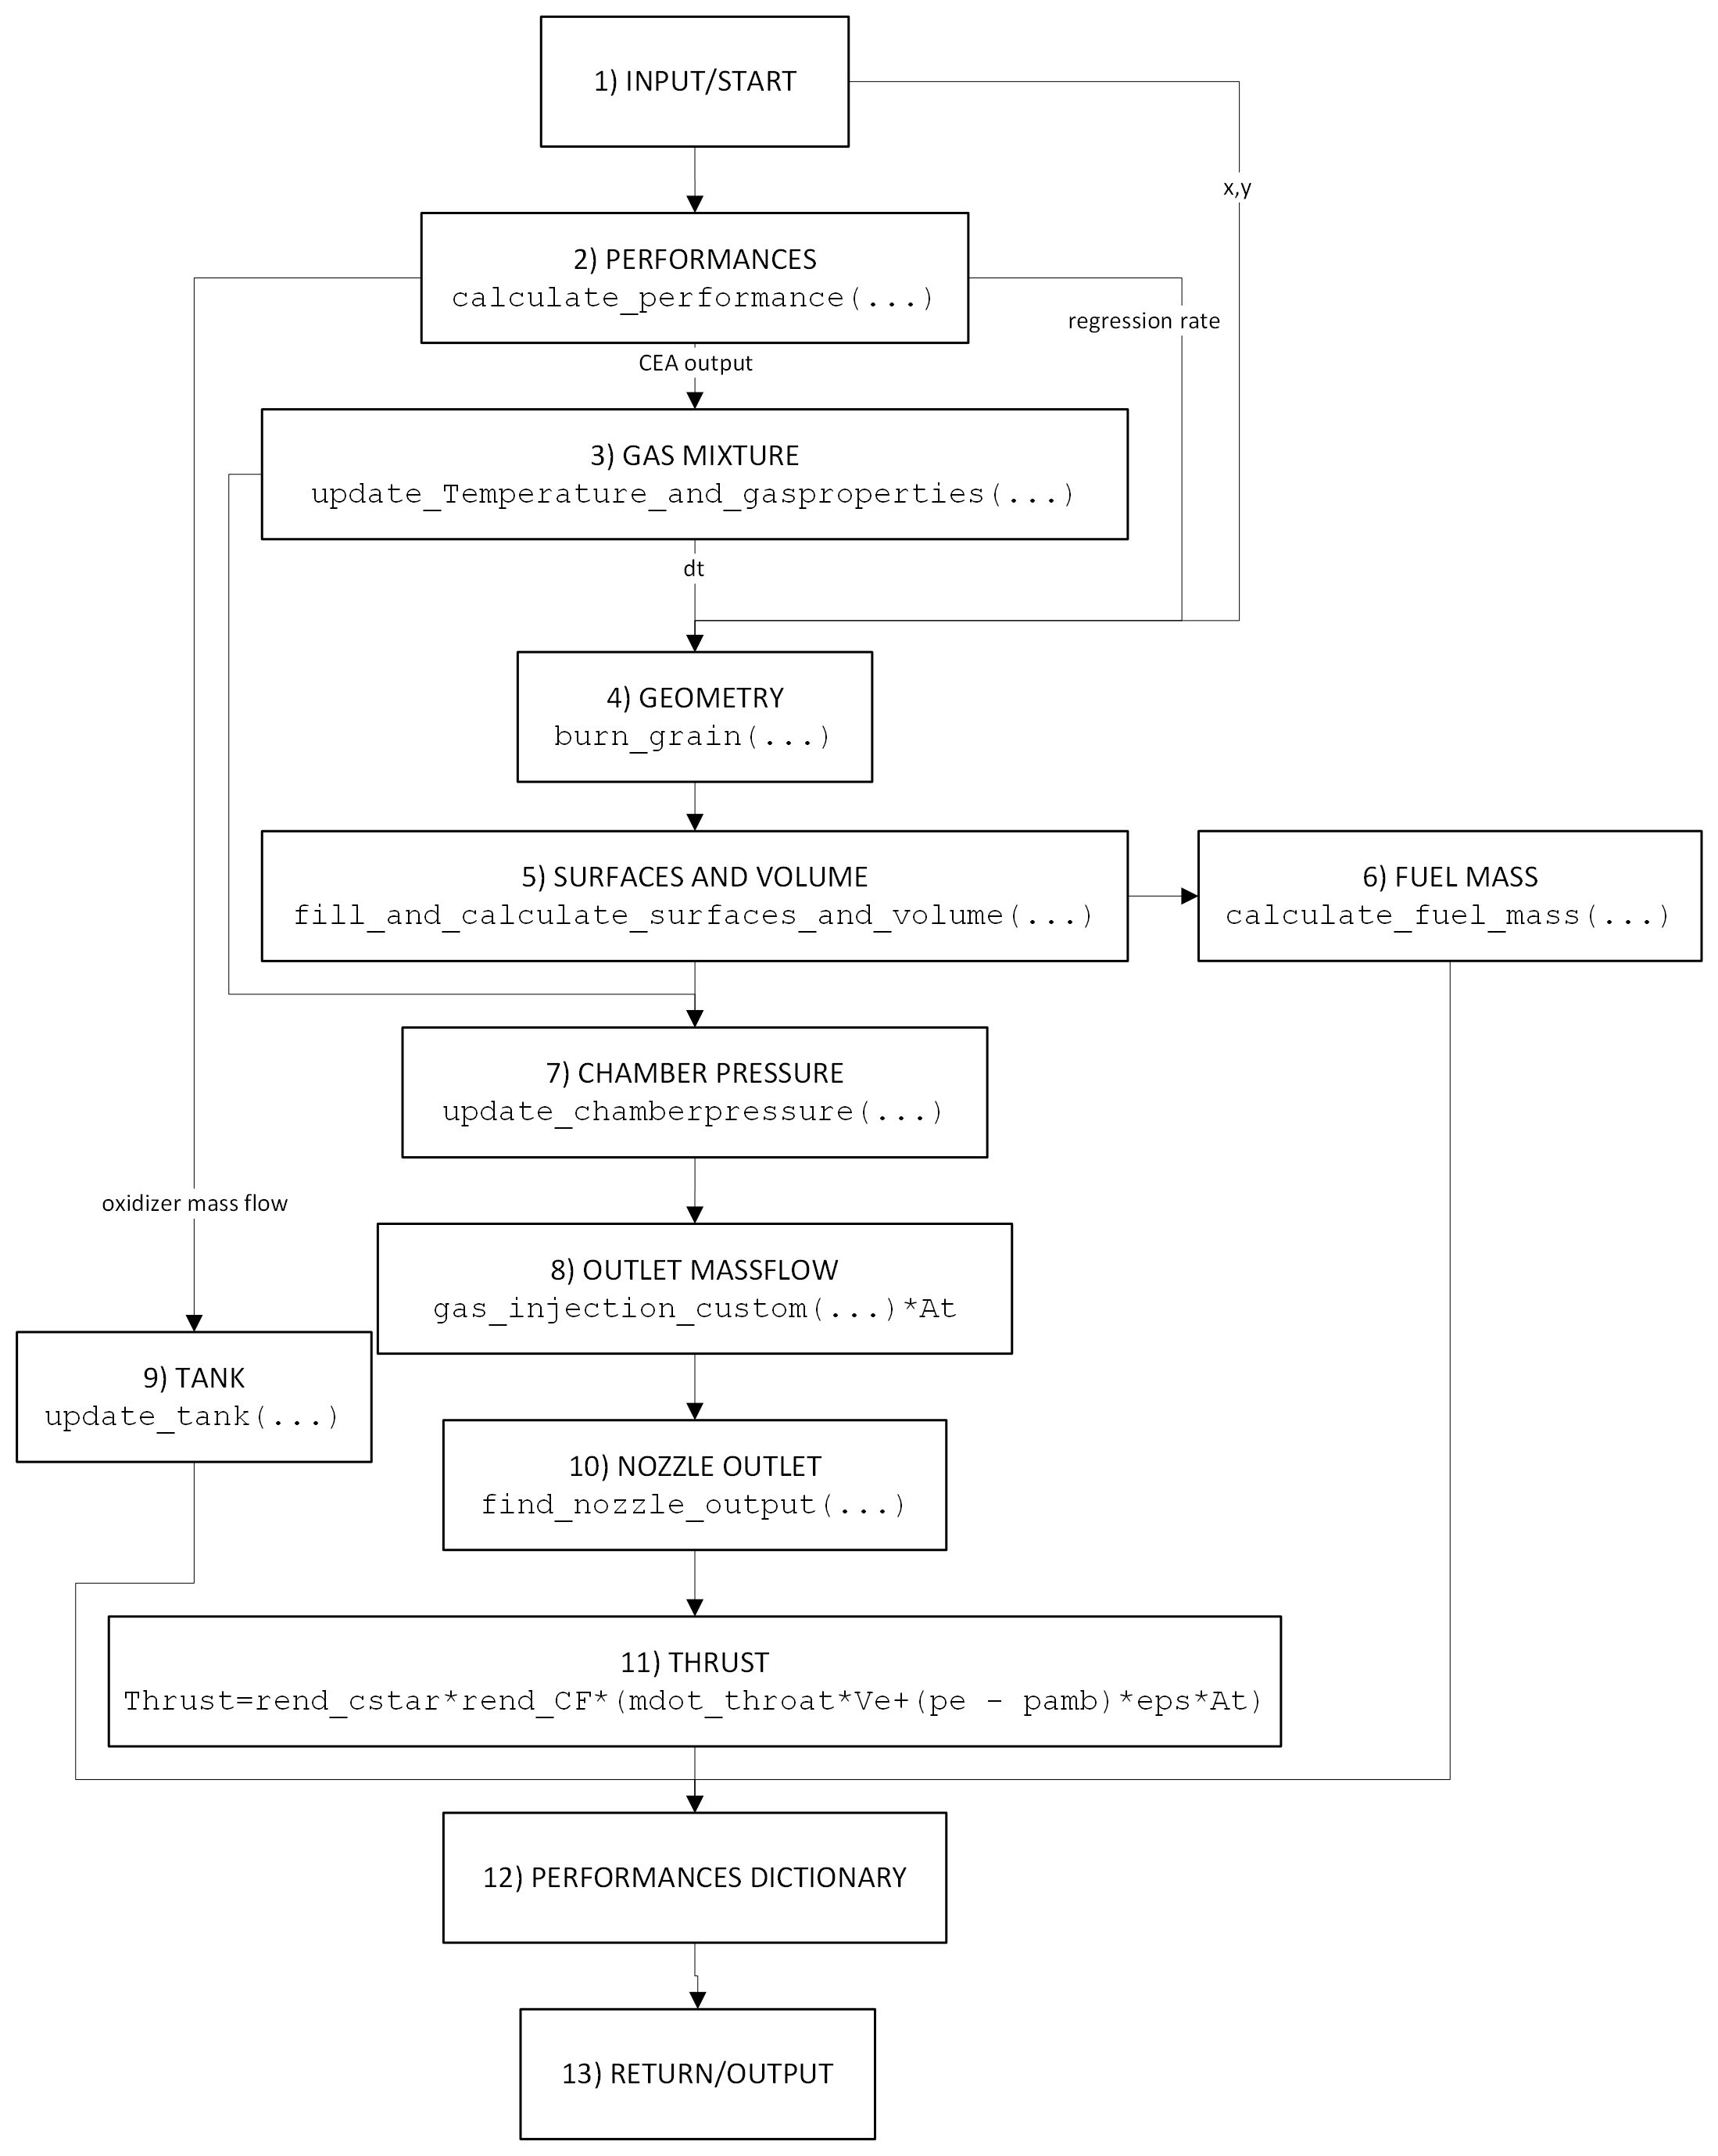
\includegraphics[width=0.9\linewidth]{immagini/burn_flowchart.png}
    \caption{Mission step flowchart}
    \label{fig:flowchartstep}
\end{figure}
The \verb|performances| dictionary is built as in Table \ref{Tab: PerfDicts}.

\begin{table}[h!]
\centering
\resizebox{\textwidth}{!}{
\begin{tabular}{|l|}
\hline
\textbf{Common values}\\
\hline
Chamber pressure "pc" [Pa]\\
Injection pressure "p\_inj" [Pa]\\
Time step "dt" [s]\\
Thrust "Thrust" [N]\\
Oxidizer massflow "mdot\_ox" [kg/s]\\
Fuel massflow "mdot\_fuel" [kg/s]\\
Total inlet massflow "mdot" [kg/s]\\
Total outlet massflow "mdot\_throat" [kg/s]\\
Chamber total temperature "Tc" [K]\\
Molecular weight "MW" [kg/kmol]\\
Specific heat ratio "gamma"\\
Expansion ratio "eps"\\
Grain points x-coordinates "x" [m]\\
Grain points y-coordinates "y" [m]\\
Port area "Ap" [m$^2$]\\
Burning area "Ab" [m$^2$]\\
Chamber internal volume "Vol\_chamber" [m$^3$]\\
Fuel mass "m\_fuel" [kg]\\
Liquid mass in the tank "mL" [kg]\\
Tank pressure "ptank" [Pa]\\
Tank temperature "Ttank" [K]\\
Exit Mach "Me"\\
Exit temperature "Te" [K]\\
Exit pressure "pe" [Pa]\\
Ambient pressure "pamb" [Pa]\\
Entropy dictionary "entropies"\\
Mass dictionary "masses"\\
Pressure dictionary "pressures"\\
Temperature dictionary "temperatures"\\
\hline
\end{tabular}
\begin{tabular}{|l|l|}
\hline
\textbf{No burn} & \textbf{Burn}\\
\hline
& Oxidizer mass flux "Gox" [kg/(m$^2$s)]\\
& Regression rate "r" [m/s]\\
& Mixture ratio "MR"\\
& Chamber temperature from CEA "Tc\_CEA" [K]\\
& Molecular weight from CEA "MW\_CEA" [kg/kmol]\\
& Specific heat ratio from CEA "gamma\_CEA"\\
& Characteristic velocity (c*) "cstar" [m/s]\\
& Thrust coefficient in vacuum "CFvac"\\
& Thrust coefficient "CF"\\
& Specific impulse in vacuum "Ivac" [s]\\
& Specific impulse "Is" [s]\\
& CEA output flag "flag"\\
Burn flag "burn": False & Burn flag "burn": True\\
\hline
\end{tabular}
}
\caption{Performance keys and values for burn and no-burn conditions.}
\label{Tab: PerfDicts}
\end{table}


